\documentclass[12pt, a4paper]{article}


% A pretty common set of packages
\usepackage[margin=2.5cm]{geometry}
\usepackage[T1]{fontenc}
\usepackage{graphicx}
\usepackage{amssymb}
\usepackage{amsmath}
\usepackage{bm}
\usepackage{color}
\usepackage{float}
\usepackage{bm}
\usepackage{physics}
\usepackage{subcaption}

\DeclareRobustCommand{\uvec}[1]{{%
  \ifcsname uvec#1\endcsname
     \csname uvec#1\endcsname
   \else
    \bm{\hat{\mathbf{#1}}}%
   \fi
}}
\newcommand{\olsi}[1]{\,\overline{\!{#1}}} % overline short italic

\usepackage[colorlinks=true, 
    linkcolor=blue,          % color of internal links
    citecolor=blue,        % color of links to bibliography
    filecolor=blue,      % color of file links
    urlcolor=blue]{hyperref}

\title{[16-833] Homework 1 : Written Report}
\author{Bharath Somayajula, Christopher Klammer}
\date{\today}

\begin{document}

\maketitle

\tableofcontents

\section{Motion Model}
TODO Chris
\section{Sensor Model}
\subsection{Sensor Model}
\subsubsection{Description}
The Sensor Model is responsible for estimating how well each particle explains the observed range sensor data. For our implementation, we followed the range sensor model described in [1] where the probability distribution of sensor measurement is modeled as a weighted average of four components that take into account randomness, presence of obstacles and errors in measurements leading to the sensor incorrectly measuring maximum range. \\\\
\begin{figure}[H]
  \centering
  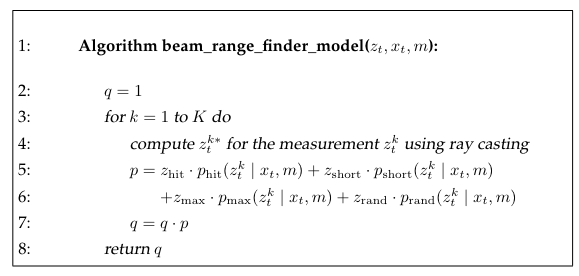
\includegraphics[width=0.9\linewidth]{results/sensor_model_desc.png}
  \caption{Description of Sensor model}
\end{figure}
The Sensor Model has been implemented in \textit{SensorModel} class in \textit{sensor\_model.py}. The constructor accepts the occupancy map and number of particles as inputs.\\\\
The function \textit{beam\_range\_finder\_model} is called from \textit{main.py} everytime a laser reading is encountered. This function performs three important tasks:
\begin{enumerate}
  \item Get ground truth range readings using ray casting module
  \item Use ground truth and sensor readings to compute probabilities of each measurement for each particle
  \item Aggregate probabilities \textit{for} each particle using sum of logarithm of probabilities for numerical stability and then normalize probabilities \textit{across} particles using softmax operation to ensure that probabilities sum to 1.
\end{enumerate}
\subsubsection{Optimization}
The \textit{SensorModel} module takes up almost all ($99.1\%$ according to our estimates) of execution time. This makes optimization absolutely essential. We made the following changes to naive implementation to speed up the code:
\begin{enumerate}
  \item We vectorized the function \textit{beam\_range\_finder\_model} and all the functions it invokes to compute probabilities of all particles at once instead of invoking the function iteratively for each particle
  \item The functions to compute the four components of probability- \textit{p\_hit, p\_short, p\_max, p\_rand} have all been vectorized to compute probabilities for all particles simultaneously. An example is shown in figure below
  \begin{itemize}
    \item 
    \begin{minipage}[t]{\linewidth}
      \vspace{0pt}
      \begin{center}
        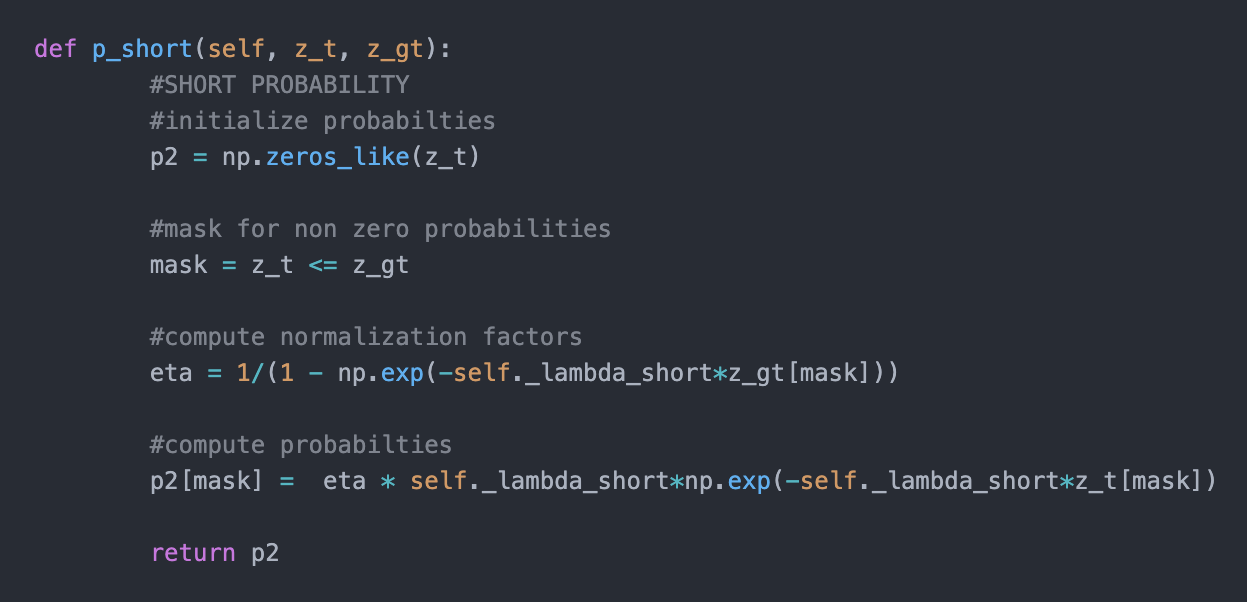
\includegraphics[scale=0.3]{./results/sensor_model_opt.png}
        \captionof{figure}{Vectorized probability computation}
        \label{fig:sm_1}
      \end{center}
    \end{minipage}
  \end{itemize}
\end{enumerate}
\subsection{Ray Casting}
\subsubsection{Description}
RayCasting is needed for estimation of true ranges at various angles.\\\\ 
To make implementation easier, we created a \textit{RayCasting} module that performs ray casting. The \textit{get\_true\_ranges\_vec} function is invoked to compute ranges at various angles for all particles.
\subsubsection{Optimization}
Ray Casting is the most computationally expensive part of the code. We implemented the following changes to naive implementation of ray casting to improve the performance.

\begin{itemize}
  \item To avoid redundant computations, we perform ray casting only once in constructor function using the \textit{relative\_ray\_casting} function. This function casts rays relative to the robot in it's canonical orientation. At all future time steps, the points along these rays are simply rotated and translated to match the position and orientation of robot! This led to massive gains in performance. The implementation of \textit{relative\_ray\_casting} function is shown below.
  \begin{itemize}
    \item 
    \begin{minipage}[t]{\linewidth}
      \vspace{0pt}
      \begin{center}
        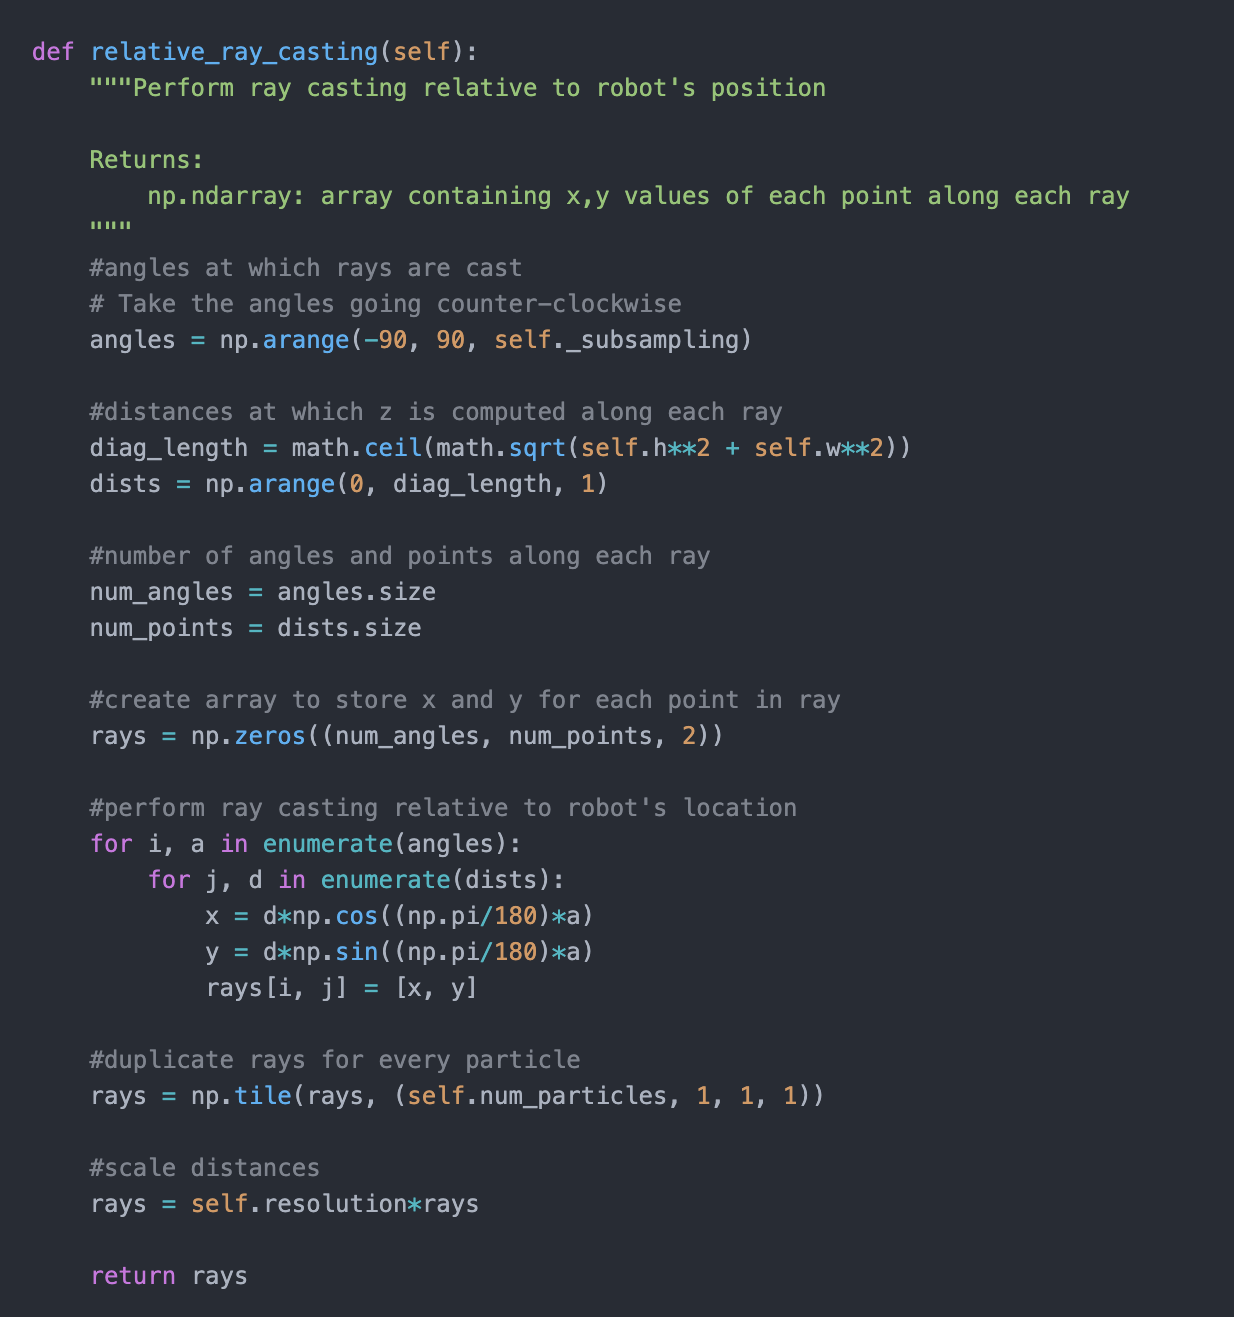
\includegraphics[scale=0.3]{./results/ray_casting_opt_1.png}
        \captionof{figure}{Pre-computation of points along rays}
        \label{fig:sm_1}
      \end{center}
    \end{minipage}
  \end{itemize}
  \item Once the rays have been oriented based on location and orientation of a particle, the logic used to measure the range along each ray at which it encounters an obstacle or goes out of the map has been vectorized. Compared to the naive implementation of this logic using nested for-loops, the fully vectorized implementation is approximately 9.5x faster.  The vectorized logic is shown below
  \item Vectorize the code to enable computation of ranges for all particles simultaneously instead of performing ray casting in a loop seperately for each particle
  \begin{itemize}
    \item 
    \begin{minipage}[t]{\linewidth}
      \vspace{0pt}
      \begin{center}
        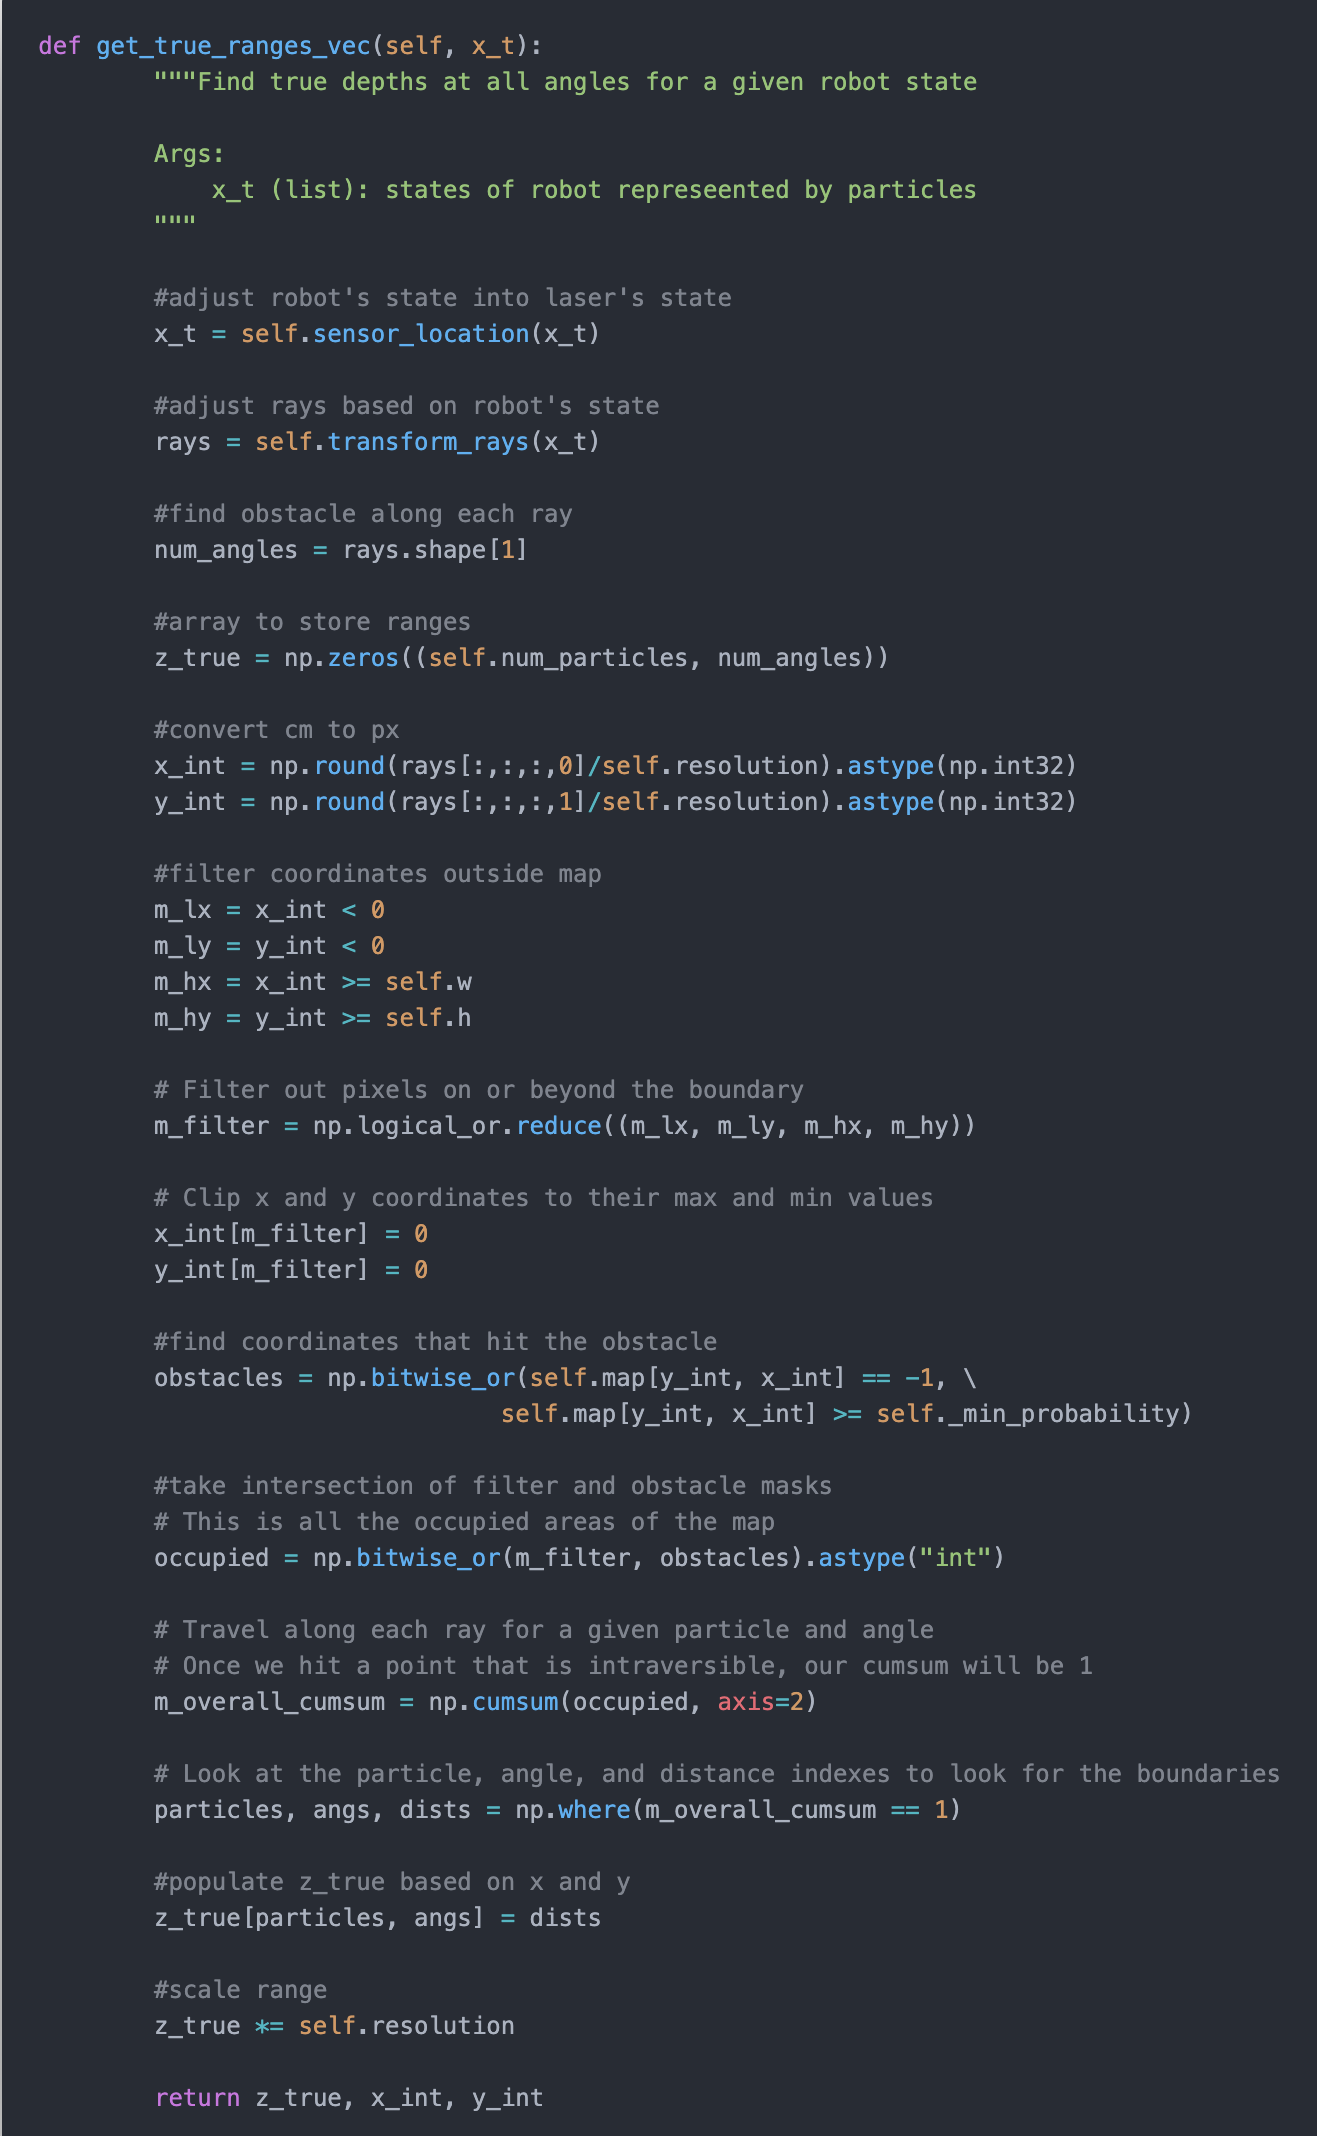
\includegraphics[scale=0.3]{./results/ray_casting_opt_2.png}
        \captionof{figure}{Vectorized logic to compute ranges}
        \label{fig:sm_1}
      \end{center}
    \end{minipage}
  \end{itemize}
\end{itemize}
The time taken to measure ground truth ranges at 36 angles for 500 particles using our optimized implementation is just around 0.5 seconds on Apple Macbook M1 Pro system.


\section{Resampling Process}
Resampling is the process by which new particles are generated from a set of modified particles and their corresponding weights.\\\\
We used low variance resampling to preserve the diversity in particle set. The figures below show the algorithm and our implementation.
\begin{figure}[H]
  \centering
  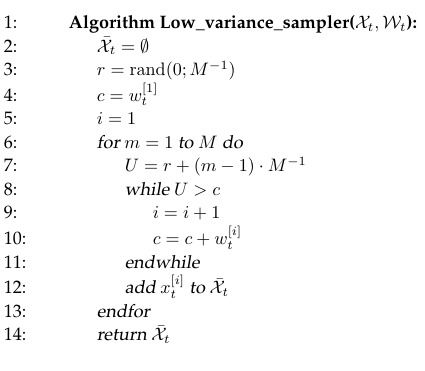
\includegraphics[width=0.9\linewidth]{results/resampling_1.png}
  \caption{Description of Resampling algorithm}
\end{figure}
\begin{figure}[H]
  \centering
  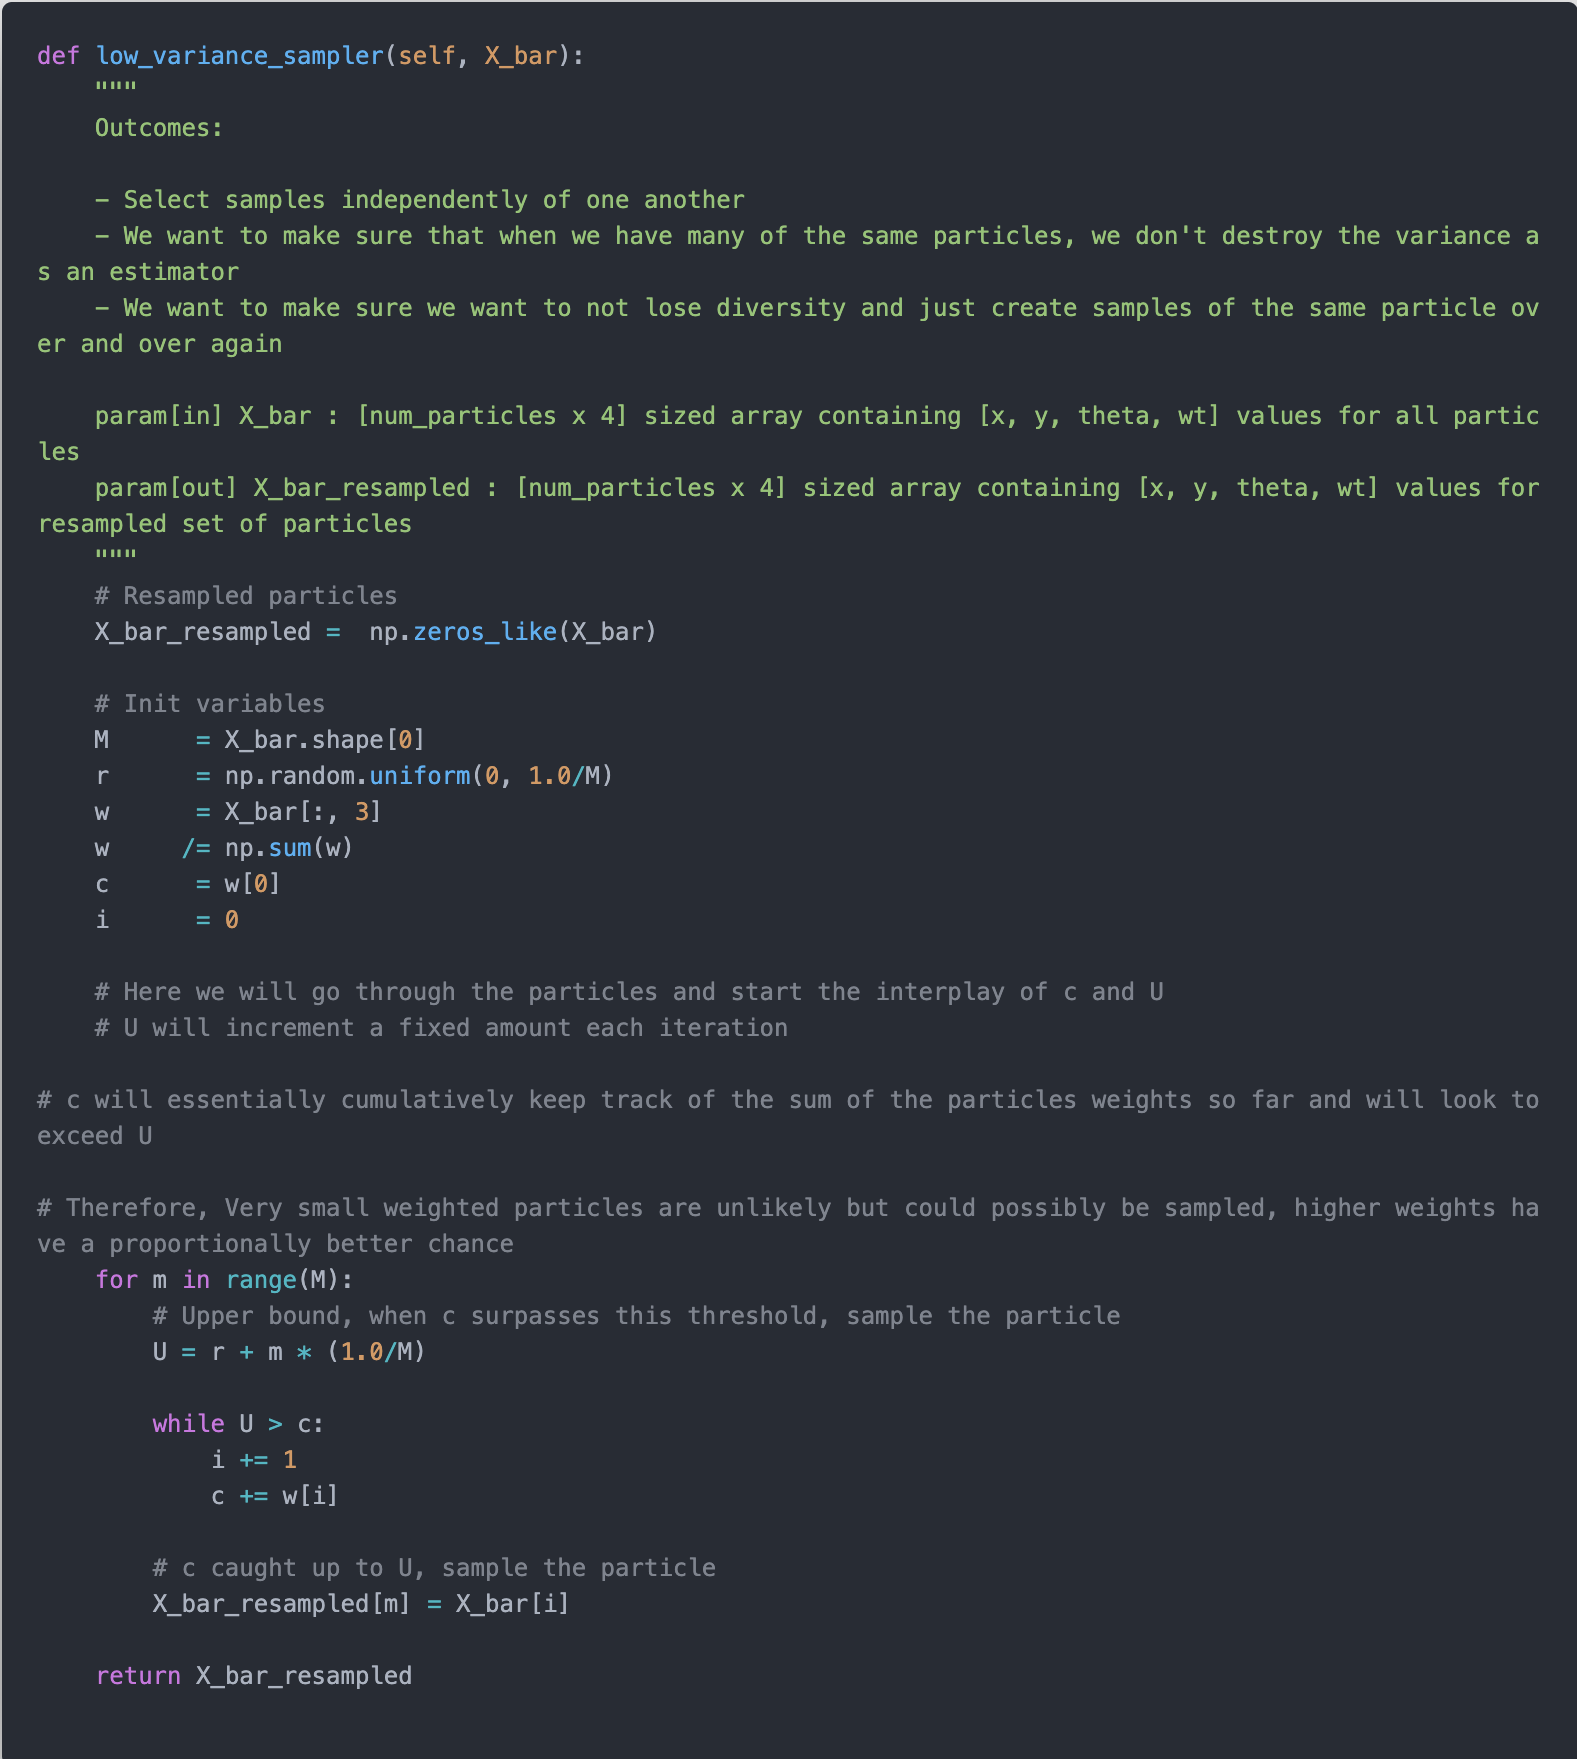
\includegraphics[width=0.9\linewidth]{results/resampling_2.png}
  \caption{Implementation of resampling}
\end{figure}

\section{Performance}
The total time taken for execution of particle filter on \textit{robotdata1.log} with 1000 particles on Apple Macbook M1 Pro is \textbf{19.6 min}. The execution time without the optimizations in ray casting is more than 3 hours(180 min).
\section{Parameter Tuning}
TODO Chris
\section{Future Work}
TODO Chris
\begin{enumerate}
  \item Implementing ray casting on GPUs that specialize in matrix multiplications and additions can further reduce the execution time of particle filter
  \item One interesting way to reduce time spent in ray casting is to approximate all obstacles in the map by a set straight lines. In this case, all the points that determine the ranges at various angles are simply intersections of any given ray and a set of lines! These points of intersection(and hence the ranges) can be computed at very little computational cost. This can potentially enable execution of particle filter in real time.
\end{enumerate}
\section{Extra Credit}
\subsection{Kidnapped robot problem}
TODO Bharath
\subsection{Adaptive number of particles}
TODO Chris

\end{document}